\documentclass{article}
\usepackage[utf8]{inputenc}

\title{CTA200H Assignment 3}
\author{Justine Obidowski}
\date{May 9th 2022}

\usepackage{graphicx}
\graphicspath{ {home/student14/Downloads/} }

\begin{document}

\maketitle

\section{Question 1}
\subsection{Methods}
\subsection{Result}

\section{Question 2}
\subsection{Methods}
\subsection{Result}

\newpage
\begin{center}
 {\title{Question 1}}
\end{center}
\\
\\
\noindent\text{Methods:}
\\
\text{A function was made to iterate the equation $zi+1 = {zi}^2 + c$ for a given number of iterations and return the value of z starting from z = 0 where c is a complex number. This function was used to calculate z values for the complex plane with -2 $<$ x $<$ 2 and -2 $<$ y $<$ 2 for chosen maximum number of iterations. The determined zi points show that some points remain bounded in absolute value while others diverge to infinity. The points that remain bounded are known as the Mandelbrot set which are the points where abs(z) $<$= 2. 
\\
\\
An image of the data was made so that the points that diverge are shown by one colour and those that stay bounded shown by another colour. This was done using for loops to go through each point of the complex plane to determine if it is bounded or not by checking if the corresponding abs(z) $<$= 2. The bounded and unbounded points were then plotted as different coloured scatter plots on the same axis.The data used was obtained from the function using a maximum iteration of 100. The plot is shown in figure 1 as an example.
\\
\\
A second image of the data was made showing points coloured by a colour scale indicating the iteration number at which points diverge.  This was done by plotting the values for abs(z) $>$ 2 (the diverging points) and using a colour bar to show the iteration number the points diverge at. This was done for a maximum iteration of 30. }
\\
\\
\title{Results:}
\begin{center}
 {\includegraphics[width=8cm]{index.pdf}}
 \\
 \text{Figure 2: Scatter plot of the points that diverge (red) and the points the are bounded (turquoise) }
\end{center}

\noindent\text{The first plot is a scatter plot which shows the points that diverge in red and the points that stay bounded in turquoise. The image shows that the bounded points are in the known shape of the Mandelbrot set which is expected.  
\\
\\
The second plot and it's color scale show that points further from the bounded points diverge at a lower number of iterations while points on or near the border regions between the bounded and unbounded points require a higher number of iterations to diverge. The plot also shows the iteration number of the bounded points as 0 as these points do not diverge.} 

\begin{center}
 {\title{Question 2}}
\end{center}
\\
\\

\noindent\text{Methods:}
\\
\text{One of the earliest known demonstrations that deterministic physical systems could exhibit behaviour that is unpredictable was given by the meteorologist Edward Lorenz when he published the paper, \emph{Deterministic Non Periodic Flow.} In this paper Lorenz introduces three differential equations: 
\\
$$ \dot{X} = - \sigma(X-Y) $$

$$ \dot{Y}  = rX - Y - XZ $$

$$ \dot{Z} = -bZ +XY $$

\\
where $\sigma$ is the Prandtl number which is the ratio of the kinematic viscosity to the thermal diffusivity, r is the Rayleigh number which depends on the vertical temperature difference between
the top and bottom of the atmosphere, and b is a dimensionless length scale. A function was made to return the results of these three equations and an ode solver was used to integrate the equations for t=60 (dimensionless time) using Lorenz's initial conditions W0 = [X0,Y0,Z0] = [0,1.,0], parameter values [$\sigma$,r,b] =  [10,28,8./3.] for 6000 iterations. 
\\
\\
The solution was then interpolated onto a time grid and the numerical solution of Y was plotted for the first 1000 iterations, second 1000 iterations and third 1000 iterations.This was done to reproduce Lorenz's figure 1 in his paper and is the first plot of the solution data. 
\\
\\
The numerical solutions to the equations were also plotted to show the projection on the YZ and XY plane in phase space of the segment trajectory extending from iteration 1400 to 1900.This was done to 
reproduce Lorenz's figure 2 in his paper. The plot obtained is shown in figure 2 as an example and is the second plot generated. 
\\
\\
A slightly different W0 was then used to find the solution of the equations. The same values of ($\sigma$, r, b) were used with the same method of solving but with initial 
condition W0' =  W0 + [0., 10$^{-8}$, 0] = [0., 1.00000001, 0.]. The distance between W' and W was then calculated as a function of time using the known distance between two points equation. The results were then plotted on a semilog plot, a plot with linear time and log distance. This plot is the third and last plot generated. 
\\
}


\\
\\
\noindent\text{Results:}
\\

\\
\noindent\text{The first plot was shown to closely resemble figure 1 in Lorenz's paper. The general pattern and shape matches for the most part but starts to slightly differ around 2000 iterations. This is likely because Lorenz used a different method to solve the equations so the results will not be precisely the same. }

\begin{center}
 {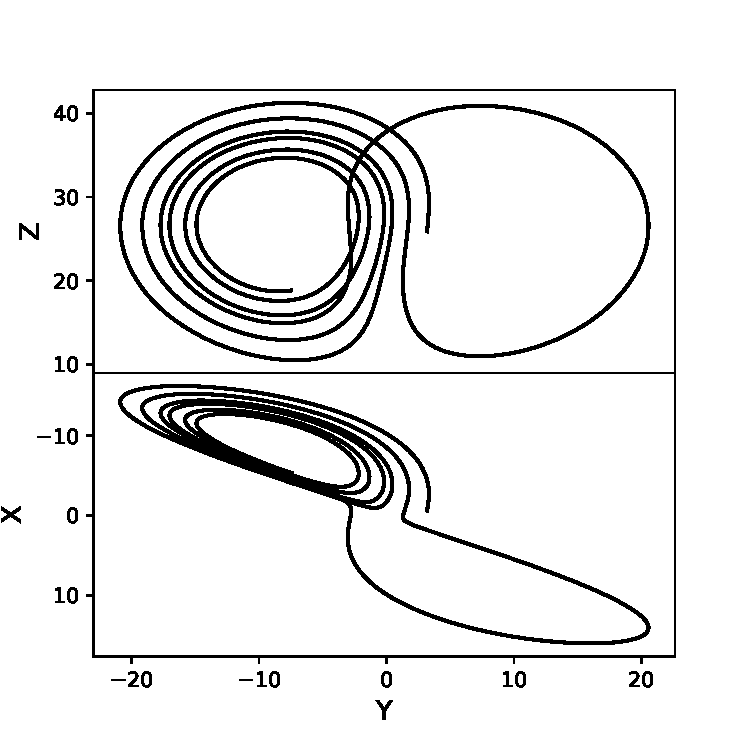
\includegraphics[width=7cm]{q2_projections.pdf}}
 \\
 \text{Figure 2: The numerical solutions to the Lorenz equations, showing the projection on the YZ plane (top) and XY plane (bottom) in phase space of the segment trajectory extending from iteration 1400 to 1900.}
\end{center}

\\
\\
\noindent\text{The second plot (figure 2) was shown to closely resemble figure 2 in Lorenz's paper. The general pattern and shape matches for the most part but starts to differ for later iterations with them falling short of their path they have in Lorenz's figure 2. This is also likely because Lorenz used a different method to solve the equations so the results will not be precisely the same.
\\
\\
The third plot was shown to have values that fluctuate somewhat linearly but the points are not quite a straight line likely due to the method of calculation. A straight is what Lorenz found which indicates exponential growth meaning the a small error in the initial condition will grow rapidly,causing predictions of future behavior will not be accurate. }

\end{document}
